% Chapter 1

\chapter{Introduction} % Main chapter title
\label{intro} % For referencing the chapter elsewhere, use \ref{Chapter1} 

%----------------------------------------------------------------------------------------

\section{Bulk RNA-seq quantification}
DNA sequencing is generally performed in three phases~\citep{schadt2010window}: fragmentation, physical-sequencing, and assembly. The first phase of fragmentation breaks the reference DNA into several small pieces and amplifies it into multiple copies, based on the requirements of the analysis. In the physical sequencing phase, individual units (called \textit{bases}) of the fragments are identified in sequential order to create a read and the number of contiguous bases in a read defines its length measured in base-pairs (bp). In the last phase of assembly, the collection of \reads (called \textit{library}) is analyzed by bioinformatics software to find overlapping regions in a \textit{library} of \reads and create "most of" the contiguous sequences of the genome. The phrase "most of" is particularly important because based on the species, sequencing technology, and many external factors, sequencing can face various different biological and computational challenges and can give different results. For example collapsing the repetitive sequence of the genome is a problem that can be solved in several ways, resulting in varying outputs.


\begin{figure*}[!htb]
\centering
\includegraphics[width=0.6\textwidth]{rapmap/{Avi.RPE.fig.4}.pdf}
\caption{From top to bottom: Single-End Sequencing, Paired-End Sequencing, information retained after Paired-End sequencing.}
\label{fig:pe-seq}
\end{figure*}


The physical-sequencing of the \reads is generally performed in one of two modes, namely single-end (SE) or paired-end (PE). To give the fragments a notion of direction as shown in~\Cref{fig:pe-seq} fragments are sequenced from 5' end to 3' end (This refers to the 5' and 3' carbons on the sugar present at each end). In SE sequencing, the fragments are sequenced only from one end. But, in PE sequencing, the fragments are first sequenced from one end for some fixed length, then from the opposite end to form a pair of \reads (called \textit{mate-pairs}). Knowing the distance between mate-pairs of a fragment in PE sequencing helps improve the specificity of the alignment of the fragment, especially when the matching region of the read in the genome is not unique. In this case, the distance between the mate-pairs can help resolve ambiguity.

Sequencing of the Human Genome~\citep{venter2001sequence} spawned many novel sequencing technologies such as 454 Life sciences (Roche), Illumina (also called Solexa Sequencing), Applied Biosystem's SOLiD, Pacific Biosciences, and Oxford Nanopore, etc. As a result of these sequencing technologies, scientists have found many biological applications for sequencing a genome, such as studying cancer (cancer genomics), gene regulatory network study and differential expression analysis, etc. Most of these biological studies require that we solve the problem of read-alignment before further analysis can be done. Moreover, the accuracy of the downstream analyses greatly depends on how well the problem of read-alignment is solved, which from a computational perspective, makes the problem of read-alignment particularly interesting. The classical problem of \ra and its general mathematical notion can be defined as follows:
\bigbreak
\textbf{Given:} A set of sequences (called \reads) $R$, a reference sequence $T$, a distance function $d(u, v)$ which gives the distance between two sequence $u$ and $v$, and $\epsilon$ (maximum edit distance) where $\epsilon \in \mathbb{Z}^{+}$.\\
\begin{equation}
\label{prboblem}
R = \{ r_i:  r_i \in \Sigma^{l_i}, \Sigma \in \{A,C,G,T\}, i \in [1, n] \}
\end{equation}
where $l_i$ is the length of the \textit{read} $i$ and $n$ is the total number of \reads.\\

\begin{equation}
T = \Sigma^k, \Sigma \in \{A,C,G,T\}
\end{equation}
where $k$ is the length of the reference sequence.\\

\begin{equation}
d:\Sigma^{|u|}\times\Sigma^{|v|}\rightarrow\mathbb{Z} 
\end{equation}

% \textbf{Exact Match Problem: \label{prb:exact}} Find $\forall r_i \in R$, a set of positions $ P = \{p : p \in \{[1, k] \cup {\phi}\footnote{\label{note1}Represents no match condition.}\} \}$ in $T$ where the sequence $r_i$ and the substring of $T$ starting at each position(s) $p \in P$, are the same.\\

\textbf{Read Alignment Problem:} Find $\forall r_i \in R$, a set of tuples $S = \{(s, p, c):  p \in \{[1, k] \cup \emptyset\footnote{\label{note1}Represents no match condition.} \} \}$ such that substring $s$ of $T$ starting from a position $p$, can be generated from $r_i$ using the transformation defined by $c$ (commonly encoded as \textit{CIGAR string}) where $d(r_i, s) \leq \epsilon$ and $c$ represents an edit script.

\bigbreak

Sequencing technology has evolved very quickly and already has three major generations of sequencers. Sanger-sequencing (First Generation sequencing)~\citep{sanger1975rapid} was developed by Sanger in 1975 and produces \reads of 1000 bp. Second-generation sequencing (SGS)~\citep{reis2009next} (sometimes called Next Generation Sequencing) technologies can produce 35bp-400bp~\citep{schatz2010assembly} \reads with very high throughput and much lower per-base cost than Sanger-sequencing. Third generation sequencing~\citep{schadt2010window}(TGS) has its advantage of read length which is tens of thousands of bp. TGS suffers from a relatively high error rate and produces comparatively fewer reads than NGS, which is important in certain applications requiring high coverage. 

The bioinformatics community has put tremendous efforts into building a wide array of different tools to solve the problem of \ra and based on the generation of the sequencer these tools use many different strategies to quickly find potential alignment for the \reads. Since the field is being explored intensively, it is very hard to discuss all the tools. We have restricted the literature of the report to SGS tools only and discussed them chronologically based on major methodological advancements over previously developed tools in their time.

\subsection{Smith-Waterman~\citep{smith1981identification}}
The Smith-Waterman~\citep{smith1981identification} algorithm is a classical algorithm for solving the problem of sequence-alignment which allows both mismatches and indels under a given scoring scheme. It guarantees finding optimal alignment under the time-bound of $\bm{O(|T|l_i)}$ for each read $r_i$ (notations as described before~\Cref{prboblem}). For a set $R$ of \reads this time-bound becomes $\bm{\sum_{r_i \in R}O(|T|l_i)}$ of which most is spent on filling DP sub-solutions that have no hope of satisfying the edit distance bound of $\epsilon$ and if we use Smith-Waterman directly on the large reference genomes (like Humans) for \ra, it becomes infeasible. The large computational cost of the algorithm and the presence of huge numbers of \reads motivated scientists to use heuristics (greedy type approach) to solve the problem.

The family of BLAST~\citep{altschul1990basic, altschul1997gapped} algorithms was one such initiative, initially designed for comparing two long sequences but used also for \ra. These algorithms attempt to optimize a specific local similarity measure which uses heuristics to give the similarity $d(u, v)$ between two sequences $u$ and $v$ based on their biological significance. BLAST gives approximate alignment results and was more than an order magnitude faster than previous methods with similar accuracy. BLAST follows a hash table based approach for preprocessing the set of \reads and a simple seed-and-extend strategy on the reference sequence to solve the problem of \ra. BLAST maintains a database of a hash table on all the k-mers (k length substrings) of the \reads and traverses the reference sequence to find a hit for seed(s) by checking the database of the hash table (called the \textit{index}). BLAST first joins the seeds without gaps and then refines them by Smith-Waterman for gapped alignment. Generally, in a big reference sequence, only a few subsequences have sufficient similarity to the query; BLAST finds these by filtering irrelevant matches using two threshold parameters $S$ and $T$. Each seed's similarity score is checked to determine if it's greater or equal to the parameter $T$. Then, BLAST tries to extend seed(s) exceeding the threshold using the Smith-Waterman algorithm to get the maximum matching score (under their similarity measure) and reports only those alignments exceeding the similarity threshold $S$.

Even though BLAST approach was faster than existing methods for read-alignment, it has some shortcomings when viewed in the context of NGS. The index needs to be built for every new read, and for alignment, BLAST scans through the entire reference sequence many times (once for each query) resulting in large computational requirements. 


\subsection{MAQ~\citep{maq}} \label{maq}
MAQ was initially developed for NGS technologies which produced tens of millions of 30-40bp \reads. With \reads this short, most genomes contain repetitive regions or nearly repetitive regions (edit distance $< \epsilon$), at least as long as these \reads. Because of the repetitive regions, \reads can align to the reference on multiple positions (called ambiguous alignments) and even a few mutations can make the read align to the wrong location. One of the major shortcomings of the \ra tools was that for better accuracy a lot of \reads are ignored based on the ambiguity of their alignment. Although conservatively discarding ambiguous \reads simplifies the read-alignment problem, it leaves out the important information from repetitive regions, which is essential for many biological applications. Instead of just ignoring ambiguous \reads, MAQ~\citep{maq} was one of the first tools to use this information. MAQ uses an approach similar to phred~\citep{ewing1998base} base-calling, i.e. not to discard the ambiguous \reads as soon as they are discovered. Instead, for each ambiguously aligned read, MAQ calculates the likelihood of the read being wrongly positioned and assigns a quality score to each alignment. Using the posterior error probability of each alignment, more information is retained than just discarding them. In a nutshell, MAQ uses a seed-and-extend type approach for aligning \reads. It builds a hash on \reads, parses the reference for a hit, but with modification in the alignment strategy of assigning a mapping quality score for each alignment (which is a measure of the confidence that a read actually comes from the position it is aligned to). Also, MAQ doesn't scan the reference sequence for every read. Instead, it builds the index on a set of reads and scans the reference a fixed (small) number of times.

To select a seed, the first 28bp of each read are hashed using six templates (12 for paired-end reads), sorted and stored in the form of a hash-table (called the \textit{index}). Then the subsequences of the reference sequence are scanned for a hit in the hash-table of all six templates. For each hit, MAQ assigns a mapping quality score, which is the sum of the qualities of the mismatching bases over the length of the whole read, extending from the initial 28bp seed without a gap and with at most 2 mismatches. Later, orphaned alignments (mate-pairs where only one mate gets aligned) are searched for gapped alignment using Smith-Waterman in the region of mapped mate-pair. The region for gapped alignments is taken to be two standard deviations of the distribution of the distance between aligned PE \reads. MAQ was also special in a sense that it utilizes the mate-pair information of paired-end \reads to correct potentially wrong alignments and accurately align \reads to repetitive sequences. The idea used by MAQ represented an important advancement but it was still far from satisfactorily solving the problem of read-alignment. For example, MAQ always reports a single alignment and in the case of equally good alignments, it randomly picks one and assigns a score of 0 (identifiable by downstream analysis). Also, no special indexing technique is used for the reference, and even for single-end reads the template hashing ensures only 2 mismatch hits, as every k-mismatch hit requires $\binom{2k}{k}$ templates. Overall, it takes 1100 CPU hours for MAQ to align 100Million 35bp PE \reads . This is still a high computational cost given the exponentially increasing pace of sequencing.

At the same time, SOAP~\citep{li2008soap} was developed to handle the problem of both ungapped and gapped alignment. Unlike MAQ, SOAP hashes the reference sequence into the memory and builds an index table for the reference sequence. It uses 2 bits per base encoding\footnote{Since we have only 4 different bases to encode i.e. A, C, T, G} to convert the read and the reference to numeric data-type and to obtain a matching score, a simple XOR of the reference subsequence with the \reads is done. It allows either a certain number of mismatches or one continuous gap for aligning a read to the reference sequence. As an example, to acquire hits with two mismatches, a read is split into four fragments and with the use of the pigeon-hole principle it made sure that at least two fragments must have no mismatches. By using all six combinations of possible fragments from a read, we can find all the hits with two mismatches. Since mismatches and gaps are not allowed simultaneously, for gapped hits SOAP uses an enumeration algorithm that tries to insert a continuous gap or deletes a fragment at each possible position in a read. In the end, the best hit for each read having a minimal number of mismatches or smaller gap is reported.  Moreover, an option for specifying the number of mismatches makes it more versatile. However, tools at this time were facing a dilemma: if an index is built on \reads, then there is overhead for scanning the whole genome many times when the number of alignments is small, but, if the index is built on the genome, then the memory requirements can become immense.

\subsection{Bowtie~\citep{bowtie}} \label{bowtie}
The next significant advancement in the world of read-alignment came with Bowtie~\citep{bowtie} which, astonishingly, at the time was able to map 25M \reads per CPU hour on the human genome using just 1.3G of memory. Bowtie's speed derived largely from using a compressed index of the reference genome. Bowtie index uses the Burrows-Wheeler transform (BWT)~\citep{burrows1994block} and FM-index~\citep{ferragina2000opportunistic, ferragina2001experimental}. The small size of the resulting index makes it possible to load it into the memory of a computer with as little as 2G of RAM. The main advantage of building the index on the reference instead of \reads is that the index can be build once and reused many times (e.g. for different sequencing experiments). Bowtie can find exact matches of any length $l$ in $\bm{O(l)}$ time and can report them all in $\bm{O(l) + k}$ time where k is number of occurrences, using the "backward search"~\citep{ferragina2000opportunistic} algorithm. For the inexact match (with mismatches) problem, bowtie essentially builds inexact alignment by finding multiple supporting exact matches.

Inexact match search (done only when no exact match is found) is performed by using the depth-first search (DFS) on the query and backtracking by replacing and inducing mismatches. Replacement is done using the minimum quality value at that base and ties are broken randomly. An exhaustive search for a read has an exponential time-bound in the number of mismatches $m$. To avoid full-length backtracking, Bowtie uses a BWT index on both the forward and reversed reference and stops backtracking after reaching the middle of the read which makes backtracking faster. The reverse reference can work well for one mismatch but is not able to avoid excessive backtracking for more than one mismatch. To prevent further backtracking, Bowtie avoids low-quality alignments by stopping backtracking at around 125 backtracks and allowing default mismatch of 2. One of the other advantages of Bowtie was that one can increase the sensitivity of the tool by increasing the default mismatch rate but with the trade-off that more time will be required because DFS will go deeper during the backtracking. 

As much as the strategy of Bowtie was novel (though similar approach was taken by SOAP2~\citep{li2009soap2}) and vastly improved the state-of-the-art in terms of running time, it started to fall short with the improvements in the sequencing throughput and read-length of the NGS, and also the launch of big research projects required much faster short-read alignment methods to handle the data analysis of large-scale sequencing experiments. With large reads ($\geq$100bp) becoming more common, Bowtie allowing any number of mismatches in the non-seed portion of the read becomes less well-suited to the data. Also, Bowtie does not allow gapped alignment which can be very important in some contexts.

Extending the concept and using the Suffix-Array (SA), BWT and FM-index; BWA~\citep{bwa} solved the problem of inexact matching by allowing gapped alignment. For exact matching, it simply finds the interval of the suffix array where the query substring occurs (which can be done in linear time using backward search~\citep{ferragina2000opportunistic}) independent to the length of the reference. For inexact matches, the process is more subtle. Given the maximum no. of indels/mismatches allowed, BWA preprocesses the query string with the BWT of the reverse (not reverse complement) of the reference. This helps BWA to avoid unnecessary backward depth-first traversal resulting in faster and accurate alignment. Many other implementation details like limiting the number of differences in the first few tens of bases of the read were done by BWA to increase the alignment rate and accuracy even further.


\subsection{BWA-mem~\citep{bwamem}} \label{bwa-mem}

In the timeline of read-sequencing, sequencers started producing Terabytes of data and handling them became tedious even for optimized tools like BWA. The need for faster methods resulted in even faster tools like \bt, BWA-mem~\citep{bwamem} and MrsFast~\citep{mrsfast}. \bt improved over Bowtie, by allowing gapped alignment using the seed and extend (difference in extension stage uses the intelligent dynamic program) approach, \bt benefits extensively from using single-instruction-multiple-data (SIMD) parallel processing to vectorize many computations. It is $\geq$ 3 times faster than BWA. BWA also continued to evolve, and BWA-mem introduced a new seed-chain-extend paradigm. In this approach, one first finds a seed for the alignment using super maximal exact matches (SMEM) based on the method of BWA, and a chain of seeds is formed based on the inter-seed distances. This often avoids useless and costly seed extension step. In the end, alignment is performed using the affine gap penalty dynamic program on the relevant chains. MrsFast is another notable tool that is cache-oblivious and indexed both reference and \reads using kmer-based approach to provide read alignments.

\begin{figure*}
 \centering
 \includegraphics[width = 1.0\textwidth]{rapmap/{Avi.RPE.fig.5}.png}
  \caption{From Top to bottom~\citep{altfigure}. : DNA, RNA and mRNA.}
  \label{fig:alt-splicing}
\end{figure*}

RNA-seq~\citep{wang2009rna} or transcriptome sequencing produces \reads from transcribed (exonic regions) regions of the RNA. As explained in~\Cref{fig:alt-splicing} first double-stranded DNA is converted to a single strand of RNA. Then, to generate mRNA from RNA different coding regions (called \textit{exon}) of the RNA are fused to form different types of mRNA ( the process is called \textit{alternative splicing}). In mRNA, the fusion point of two different exonic regions of the RNA is called as \textit{splice junction}. If \reads from RNA-seq are aligned to the genomic reference sequence, a read can map to splice junction of mRNA which in the genomic region could be tens of thousands of bases apart and current methods of read-alignment will fail.

This divided the alignment problem into two different regimes namely spliced aligners and unspliced aligners. Spliced read aligners try to solve the problem of aligning to a target reference genome where some \reads can span exons junctions. These tools are called splice read aligners since they have to find alignments to exon-exon junctions which maybe tens of thousand bases apart in the reference. On the other hand, they typically encounter very little multi-mapping since most \reads have a single genomic locus of origin. Some of the notable spliced aligners are like TopHat~\citep{trapnell2009tophat}, \STAR~\citep{star}, Subread aligner~\citep{liao2013subread} which use novel seed and vote strategy and the recently published HISAT~\citep{hisat} which uses a hierarchical FM index to allow very fast mapping of both DNA-seq and RNA-seq \reads with only small memory requirements. 

\begin{table*}[hbtp]
\centering
\caption{Short-Read Aligners/Mappers property. MAQ represents if mapping quality is used by tool or not}
\label{tab:aligner_property}
\begin{tabulary}{2cm}{lrrrr}
\toprule
% {} & \multicolumn{4}{c}{Flux simulation} & \multicolumn{4}{c}{RSEM-sim simulation} \\
% \midrule
Tool &   Indexing  &  Gapped  &  Paired-end &  MAQ\\
\midrule
BLAST   &      hash \reads          &          No     &   No    & Yes\\
MAQ     &      hash \reads         &          Yes     &   Yes & Yes\\
SOAP     &      hash reference     &          Yes     &   Yes    & Yes\\
Bowtie  &      FM-index         &          No     &   Yes    & No\\
BWA     &      FM-index         &          Yes     &   Yes    & No\\
BWA-mem &       FM-index            &           Yes    &    Yes    & No\\
pseudo-mapping & T-DBG            &           Yes    &    Yes    & No\\
\qm        &       Suffix Array        &           Yes    &    Yes    & No\\
\bottomrule
\end{tabulary}
\end{table*}

Transcriptome aligners are same as unspliced aligners (i.e. they work on transcriptome level) but they also intelligently handle high multi-mapping rate in the alignments due to the presense of isoforms of the same exonic regions in mRNA. As can be seen in~\Cref{fig:alt-splicing}, \textit{exon1} (in blue) is present in all the mRNA and if a read is generated from the region of exon1 from any one mRNA it'll get aligned to each of them equally well. The modified problem of \ra for transcriptome aligners can be defined as follows:

\bigbreak
\textbf{Given:} A set of sequences (called \reads or RNA-seq \reads) $R$, a set (called transcriptome) $T$ of reference sequences (called transcripts) $t$, a distance function $d(u, v)$ which gives the distance between two sequence $u$ and $v$, and $\epsilon$ (maximum edit distance) where $\epsilon \in \mathbb{Z}^{+}$.\\
\begin{equation}
R = \{ r_i:  r_i \in \Sigma^{l_i}, \Sigma \in \{A,C,G,T\}, i \in [1, n] \}
\end{equation}
where $l_i$ is the length of the \textit{read} $i$ and $n$ is the total number of \textit{reads}.\\

\begin{equation}
T = \{ t_i:  t_i \in \Sigma^{\ell_{t_i}}, \Sigma \in \{A,C,G,T\}, i \in [1, k] \}
\end{equation}
where $\ell_{t_i}$ is the length of the transcript $i$ and $k$ is the total number of transcripts.\\

\begin{equation}
d:\Sigma^{|u|}\times\Sigma^{|v|}\rightarrow\mathbb{Z} 
\end{equation}

% \textbf{Exact Match Problem: \label{prb:exact}} Aim is to find $\forall r_i \in R$ if possible, a set of tuple $ P = \{p, t_y : p \in [1,lt_y], y \in [1, k]\}$ in $T$ where the sequence of $r_i$ and the subsequences of $t_y$ at the location $p$ , are exactly the same.\\

\textbf{Read Alignment Problem for Transcriptome: \label{prb:inexact}} Find $\forall r_i \in R$, a set of tuple $S = \{(s, p, t, c):  p \in \{[1, k] \cup \emptyset\footnote{\label{note1}Represents no match condition.} \} \}$ such that substring $s$ of transcript $t$ starting from a position $p$, can be generated from $r_i$ using the transformation defined by $c$ (also called \textit{CIGAR string}) where $d(r_i, s) \leq \epsilon$ and $c$ represents a collection of match, mismatch, insertion and deletion (indel).
\bigbreak

Transcriptome aligners focus primarily, on a different problem from spliced-aligners (though some of the spliced aligners can be used as transcriptome aligner) since they have to align \reads to the transcriptome instead of the genome. Specifically, they face a huge rate of multi-mapping in \reads but they don't have to handle spliced events (since they assume a reference that consists of the already spliced (i.e. mature) transcripts). Transcriptome alignment can also be used after \denovo transcriptome assembly and does not rely on the knowledge of the reference genome of the organism. ~\Cref{tab:aligner_property}~\citep{li2010survey} gives a gist of some of the tools and their constituent properties.

\subsection{Salmon~\citep{salmon}} \label{salmon}

\salmon solved an important problem of quantification by using a novel concept of lightweight-alignemnt~\citep{salmon}. The main motivation behind lightweight alignment was the realization that in some special biological application (in the case of \salmon it was the quantification of transcript abundances from RNA-seq \reads), we do not require the actual alignment between the query sequence (i.e. $c$ in our problem formulation) and the reference. Rather, simply knowing the transcripts (and the position in that transcript) where each match reasonably well is sufficient to solve the problem. \salmon attempts to find these mapping locations using BWA-mem type seed-chain-extend approach i.e. seeding through SMEM, chaining MEM and SMEM together and extending it to only exact matches.

The introduction of lightweight-alignment further divided the transcriptome aligners into two different regimes, namely aligners and mappers. Aligners (as discussed in ~\Cref{prb:inexact}) work by generating a CIGAR string which is a base-to-base correspondence between two query strings. But, in comparison to alignment, mappers do not find CIGAR strings. Instead for each read $r_i$, they just report transcript $t$ and the position $p$ in $t$ where $r_i$ gets aligned “sufficiently well”~\citep{blog}\footnote{Since the problem is less well-studied than alignment and a reasonable determination of what constitutes “sufficiently well” is still a reasonable topic for discussion and debate}.

Using a different, alignment-free approach, a recent quantification tool \kallisto~\citep{kallisto} makes use of Transcriptome-de-Bruijn graph(T-DBG) to compute called pseudo-alignments. \kallisto builds a de-Bruijn graph on the transcriptome and labels each unique k-mer region on the graph with its constituent transcripts. During the pseudo-alignment stage, a procedure is used to extract a subset of k-mers from the read and intersect them with the T-DBG to determine a "compatible" set of transcripts. In some sense, pseudo-alignment goes even further than mapping in that the pseudo-alignments themselves give no information about where (position) or how (orientation) a read maps to a transcript (though pseudo-alignments can be pre-processed, at some extra cost to approximate this extra information). The field of read-mapping is under constant development and we have developed a novel mapping technique, called \qm, using the suffix array, which is discussed in \cref{rapmap}.

\section{Single Cell RNA-seq quantification} 
\label{intro:singlecell}

Bulk RNA-sequencing is an established method to perform genome-wide quantification of gene expressions \citep{mortazavi2008mapping}. However, bulk experiments average-out the expression pattern of an individual cell (or a cell type) across the full experiment -- typically millions of cells, losing cell-level heterogeneity which is crucial, for example, to understand the Waddington landscape of an epigenomic analysis ~\citep{goldberg2007epigenetics}. Shortly after bulk RNA-seq experiments became common, \citet{tang2009mrna} proposed single-cell RNA-seq (scRNA-seq) to perform a transcriptome-wide study of single cells. Even though it was restricted to investigating a few interesting cells, it later allowed exciting biological and medical insights such as characterizing cellular states and molecular circuitries \citep{encode2012integrated}. Since then, many \singlecell protocols have been proposed which improve many aspects of the technology; for example in \Cref{fig:sc-techs} \citep{svensson2018exponential} show the exponential scaling of single-cell RNA-seq in the past decade, enabling the characterization of transcriptional profile for thousands or even millions of single cells.

In general, \singlecell protocols follow similar library preparation steps. As shown in \Cref{fig:libprep} and discussed by \citep{ziegenhain2017comparative}, it requires the isolation and lysis of single cells, the conversion of their RNA into cDNA, and the amplification of cDNA to generate high-throughput sequencing libraries. However, along with the monetary cost, the effectiveness of single cell protocols is determined by a number of diverse variables like technical factors such as the rate of cell isolation (i.e. the fraction of cells in the population which is picked up), sensitivity to capture mRNA molecule in a cell and conversion to cDNA molecule, or the rate and the accuracy of the amplification procedure used by the single cell technology. Although the technical possibilities are vast, the main limiting factors for \singlecell technologies include financial considerations and the larger amount of biological material required to start an experiment \citep{vieth2017powsimr, ziegenhain2017comparative}. These factors limit the statistical power of an assessment and motivate more involved method development to process the data generated through these single-cell protocols.



\begin{figure*}
 \centering
 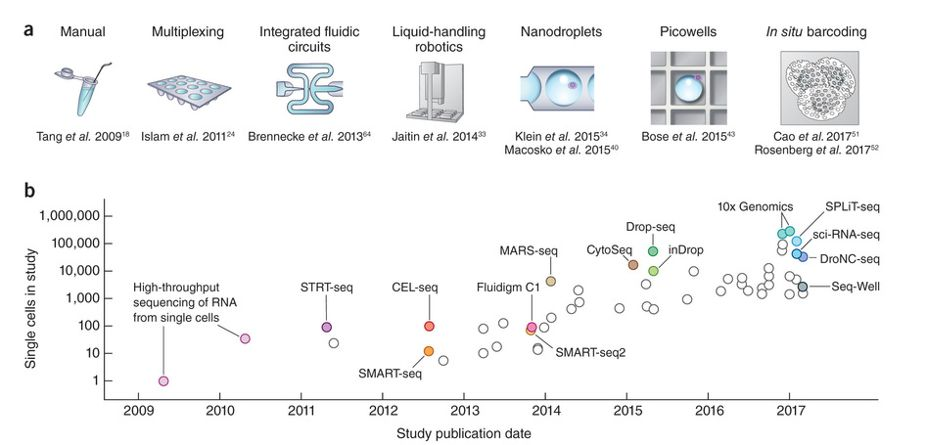
\includegraphics[width = 1.0\textwidth]{alevin/tech_progress.jpg}
  \caption{Scaling of scRNA-seq experiments \citep{svensson2018exponential}}
  \label{fig:sc-techs}
\end{figure*}

\begin{figure*}
 \centering
 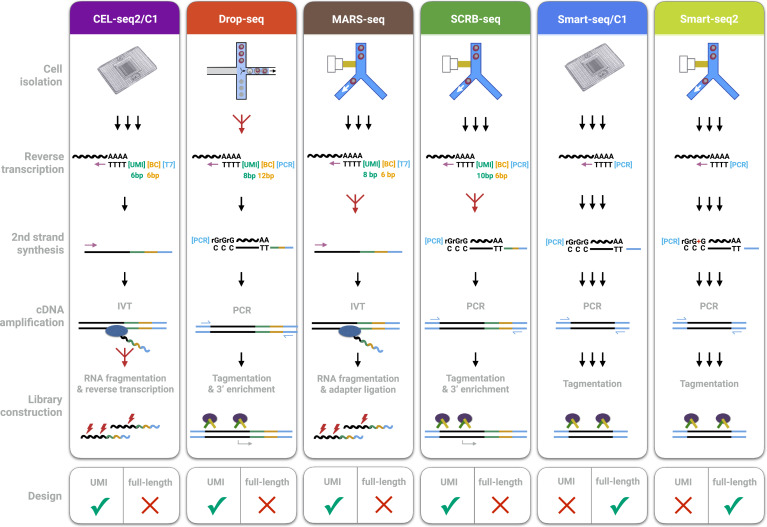
\includegraphics[width = 1.0\textwidth]{alevin/libprep.jpg}
  \caption{Schematic Overview of Library Preparation Steps \citep{ziegenhain2017comparative}}
  \label{fig:libprep}
\end{figure*}

\subsection{Fluidigm based platforms ~\citep{islam2012highly, hashimshony2012cel}}
\label{intro:fluidigm}

One of the earliest techniques to capture and isolate single cells was based on microliter volume plates (microwell plates) \citep{islam2012highly, hashimshony2012cel}. Later it was automated through the microfluidic platform from Fluidigm (C1 platform) \citep{islam2014}, typically in very small volumes of a few nanolitres. The platform uses an integrated fluidic circuit (IFC) array where a batch of cells is loaded through pipetting. The microfluidics system in the platforms separates the cells into different chambers which are called as wells. The earlier C1 platform uses a 96 well plate but more recently an 800 well plate has also been available by Fluidigm. The C1 platform after capturing individual cells automatically washes and lysis, perform reverse transcription and PCR amplify the collected cDNA, which is extracted and sequenced through Illumina sequencing.

The C1 platform has provided a range of opportunities for many experiments but has its limitations. Some of the caveats associated with Fluidigm based experiments include relatively low throughput, in expectation higher per-cell cost, and the size of ICF chip as it captures cells of a particular size in a single run. In contrast to plate-based capture methods, which usually provide reads along the full length of a molecule, an alternative droplet-based capture method \citep{dropseq, indrop, tenx} was proposed which trades-off full-length sequencing with higher throughput resulting in lower per cell cost. In this study, we are going to focus primarily on droplet-based single-cell RNA-sequencing (dscRNA-seq).

\subsection{Droplet based platforms ~\citep{dropseq, indrop, tenx}} 
\label{intro:droplet}
Droplet-based platforms work by capturing cells in nanoliter-sized aqueous droplets by associating a different barcode with each cell’s RNAs and sequencing them all together. Initially, droplet-based platforms were released as DIY systems but later automated and commercialized by 10x Genomics ~\citep{tenx} and their chromium platform.
As discussed by ~\citet{lukesthesis}, all three platforms work in a similar fashion apart from how the beads are produced, when the droplets are broken and in some aspects of their chemistry. In ~\Cref{fig:dropprep} we show how the molecular barcoding is performed in one of the dscRNA-seq platforms as proposed by ~\citep{dropseq}. In the drop-seq platform, individual cells are dissociated from complex tissue and along with a flow of beads, suspended in lysis buffer, are encapsulated into nanoliter-sized emulsion droplets. Inside the droplet, the cells are lysed and its mRNAs bind to the primers on the droplet's companion microparticle which is reverse-transcribed into cDNAs generating a set of beads. The droplets later break generating a library for all cells in parallel in one single tube which is amplified in pools for high-throughput Illumina sequencing. 

\begin{figure*}
 \centering
 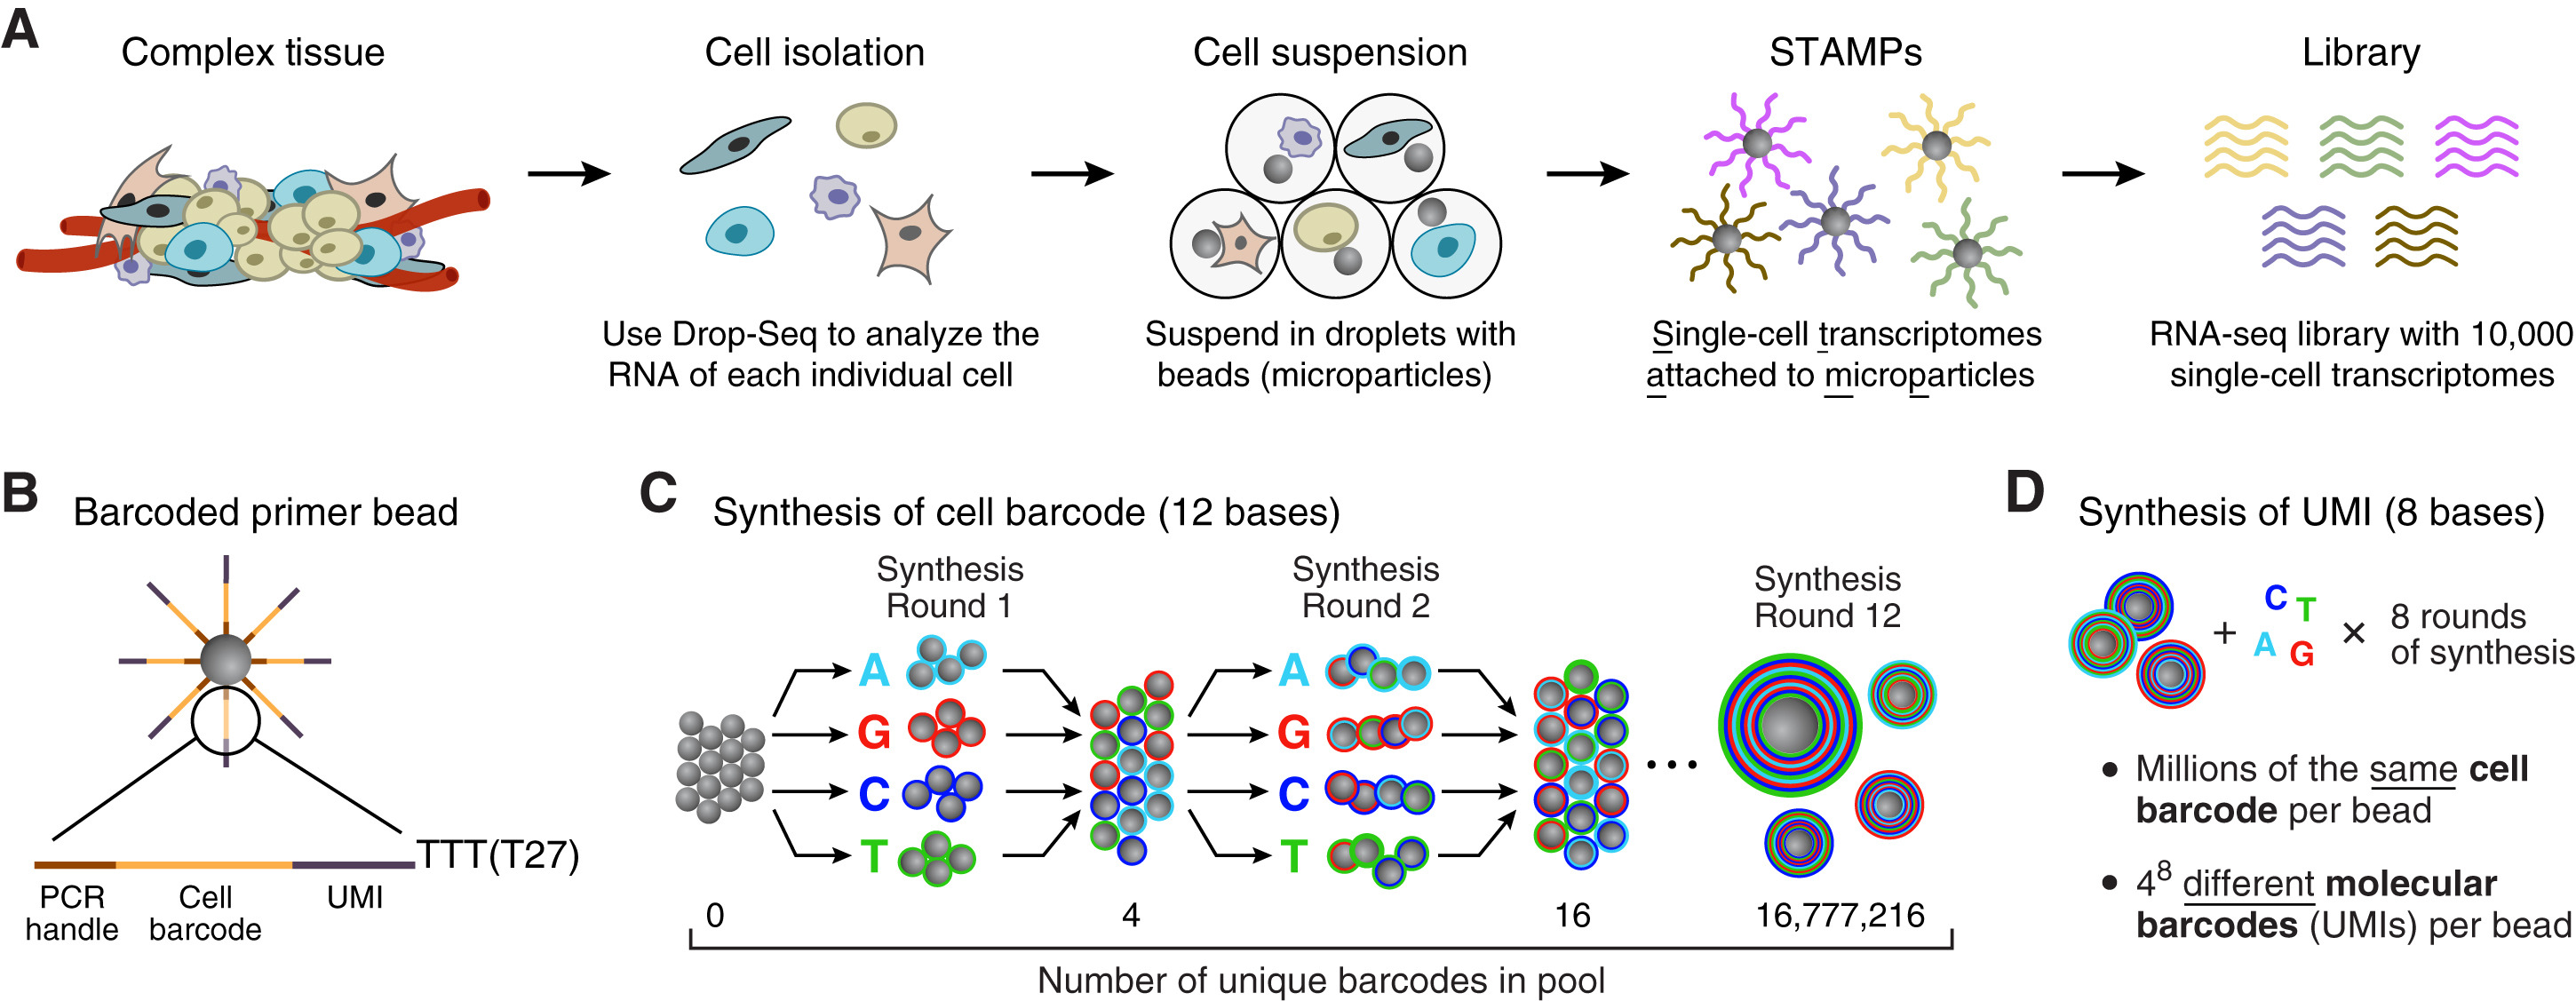
\includegraphics[width = 1.0\textwidth]{alevin/dropseq.jpg}
  \caption{Molecular Barcoding of Cellular Transcriptomes in Droplets \citep{dropseq}}
  \label{fig:dropprep}
\end{figure*}

On each bead, oligo-dT primers have a covalently bounded UMI (Unique Molecule Identifier) and a unique, bead-specific cellular barcode (CB). Association of each individual molecule with a cell-unique UMI sequence before PCR amplification makes the platform particularly effective as only a small section at the 3' end of each molecule is sequenced. This has a monetary benefit of reducing the amount of cDNA that needs to be sequenced and therefore increases the number of cells that can be sequenced at a time, at a similar cost. However, the trade-off of the coverage with throughput comes at a cost of making this platform unsuitable for applications such as variant detection and de-novo assembly. Moreover, traditional pipelines for bulk RNA-seq quantification also cannot be directly used for dscRNA-seq quantification as datasets with CB/UMI need extra processing steps like CB whitelisting (the process of disambiguating droplets with real cells from empty/doublet containing droplets), UMI deduplication (the process of modeling PCR tree to deduplicate UMI sequences) which are non-trivial to model efficiently.

A typical dscRNA-seq experiment contains a very small amount of RNA ($\sim$ 10--30 pg) of which less than 5 percent of which is mRNA ~\citep{lukesthesis}. The tiny sample size makes it difficult to process and necessitates a PCR amplification step, however, the rate of amplification of each molecule in each cell is not controllable and creates an irregularity in the expression of the transcript and gene abundances. Along with CB whitelisting, a basic model of PCR tree for deduplication has been previously applied by various protocols ~\citep{dropseq, tenx}. In ~\Cref{alevin}, we propose a unified pipeline called \alevin where we describe an end-to-end quantification pipeline that takes as input sample-demultiplexed \texttt{FASTQ} files and outputs gene-level UMI counts for each cell in the library.